
\pagenumbering{arabic}
\newpage
\section{Introdução} % (fold)
\label{sec:introducao}

% roteiro introdução:
% paragrafo1: apresentar o cenário do verão de 2014, falar do giro anticiclonico
% paragrafo2: explicar a origem do bloqueio: pode colocar imagem do CPTEC
% paragrafo3: pq o tema é interessante e bacanudo ? 
% paragrafo4: importancia de compreender a dinâmica frente a um novo regime de vento predominante
% importância no meu caso pode estar relacionado às mudanças climáticas e aumento dos eventos deste fenômeno, influenciando a circulação local por um longo período de tempo. com isso, a navegação e diversas outras atividades [a pensar] seriam impactadas.

%%%%%%% ROTEIRO INTRODUÇÃO
% Primeiro parágrafo, ideias gerais: CENÁRIO ATMOSFÉRICO COMUM DO AS: ASAS/SISTEMAS FRONTAIS + mudanças
% inicio: localização da PCSE no mundo + padrões atmosféricos que controlam o regime de ventos da PCSE: a ASAS e os sistemas frontais
% medio: mudança da posição da asas e bloqueio da migração dos sistemas frontais associados a essa mudança
% final: consequências: baixa precipitação + TSM elevada
\hspace{6mm} A Plataforma Continental Sudeste (PCSE) está localizada a oeste do Atlântico Sul. 
Tem como principais responsáveis na geração de movimento ventos de nordeste e leste, associados a 
Alta Subtropical do Atlântico Sul (ASAS), e ventos de sul, associados aos Sistemas Frontais
de Mesoescala (frentes frias) \shortcite{Castro1998}. O centro da ASAS está localizado, em
média, em 30$^o$S 10$^o$W. Entretanto, no verão de 2014 houve um bloqueio atmosférico, impedindo 
a migração de frentes frias \shortcite{Rodrigues2017}. Este período foi marcado por altas temperaturas da superfície do mar, 
que contribuíram para os baixos índices de precipitação observados. Durante este evento, os reservatórios 
de água que abastecem cidades como São Paulo e Belo Horizonte, alcançaram níveis críticos, 
ocasionando a crise hídrica da região sudeste brasileira em 2015 \shortcite{Coelho2016a}.

% Segundo parágrafo, ideias gerais: bloqueio atmosférico da ASAS e aumento destes nos ultimos anos
% inicio: como são formado bloqueios atmosféricos da ASAS
% medio: pq acontecem e quando ocorrem (impacts of atmospheric blocking on south ...)
% final: aumento destes nos últimos anos
\hspace{6mm} O bloqueio atmosférico ocorrido no verão de 2014 foi causado por uma 
fonte de calor na Austrália, que intensificou as perturbações na atmosfera, eventualmente
quebrando anticiclonicamente na região sudeste brasileira. Devido a estabilidade dos giros
anticiclônicos, estes bloqueios duram de dias a semanas, com raros casos de 
duração por mais de 15 dias. Dentre estes casos, destaca-se o o verão do ano citado,
onde foram mais de 45 dias de bloqueio na região sudeste, sendo que um único 
evento ocorreu por 30 dias (de 15 de Janeiro a 13 de Fevereiro) \shortcite{Rodrigues2017}.

% Terceiro parágrafo, ideias gerais: mudanças no padrão de ventos da pcse
% inicio: novos ventos predominantes por longo período de tempo
% medio: embasamento teórico para tempo que o vento precisa agir para influenciar circulação superficial
% final: 
\hspace{6mm} Embora haja períodos em que os ventos predominam de Sul na PCSE, o tempo de 
influência deste regime não passa de alguns dias, durante a passagem das frentes frias.
Entretanto, durante o verão de 2014, os ventos associados ao sistema que antes eram de Leste e 
Nordeste, passam a ser de Sudoeste, agindo na região costeira por um longo período, como 
pode ser observado na Figura~\ref{fig:a701}, onde a direção e intensidade do vento 
obtida no \textit{Climate Forecast System Version 2} (CFSv2), durante o período de 
01 de Dezembro de 2013 a 28 de Feveiro de 2014. Nota-se que a direção
predominante neste período é do terceiro quadrante (S/SW).

\hspace{6mm} Com essa mudança no regime de ventos predominante neste 
cenário, a circulação conduzida pelo vento na plataforma muito provavelmente sofreu alterações.
Frente a importância da PCSE, tanto no aspecto de navegação, quanto de
exploração e uso das águas e considerando que as mudanças climáticas poderão 
influenciar a frequência de eventos de deslocamento da ASAS, é importante compreender 
como a dinâmica da circulação será afetada sob a influência de novos regimes
de vento.

\begin{figurehere}
  \centerline{\hbox{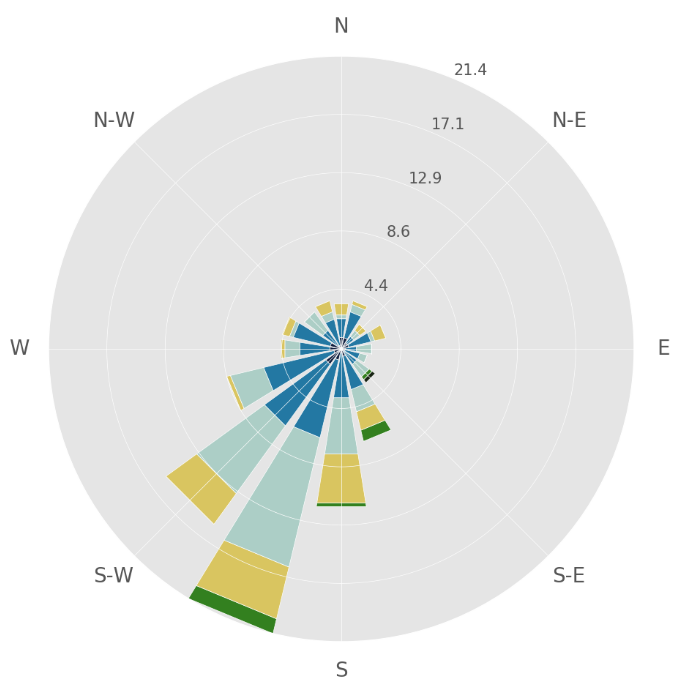
\includegraphics[height=4.in]{/home/danilo/Documents/mestrado/ventopcse/figuras/windrose_2014CFSv2.png}}}
  \vspace{-.1in}
  \caption{Rosa dos ventos para ventos a 10 metros de altura da superfície, extraídos do \textit{Climate Forecast System Version 2}
  (CFSv2), para o período de Dezembro/2013 a Feveiro/2014, utilizando-se a conveção meteorológica.}
\label{fig:a701}
\end{figurehere}
\bigskip

\subsection{Área de Estudo}
\label{sub:areaestudo}

\hspace{6mm} A área de estudo deste trabalho está localizada na Margem Continental
Sudeste Brasileira, compreendida entre o Cabo de Santa Marta, ao Sul, e pelo
Cabo Frio, ao norte. Esta região possui uma extensão de 1.100km e largura variando de 230km, ao
largo de Santos, a 50km na extremidade norte (Cabo Frio). A quebra da plataforma
ocorre em uma profundidade entre 120 e 180m, possuindo uma declividade suave. 

% \textbf{falar das isobatimetricas paralelas a linha de costa e da presença
% da Corrente do Brasil no talude}

\hspace{6mm} A estrutura termohalina da PCSE é classificada pela interação entre
três massas d'água: Água Costeira (AC), Água Central do Atlântico Sul (ACAS) e
Água Tropical (AT) \cite{Castro1987}. A partir da observação destas estruturas,
\shortciteN{Castro1996} caracterizou duas frentes na Plataforma Continental Norte
de São Paulo (PCNSP): Frente Térmica Profunda (FTP) e Frente Halina Superficial (FHS).
A partir dos parâmetros das duas frentes e das propriedades físicas das massas
d'água, o autor propôs a divisão da PCNSP em três compartimentos:

\begin{itemize}
    \item Plataforma Continental Interna (PCI), entre a costa e a FTP;
    \item Plataforma Continental Média (PCM), entre a FTP e a FHS e
    \item Plataforma Continental Externa, entre FHS e a quebra da plataforma continental.
\end{itemize}

\hspace{6mm} As correntes da PCI são forçadas pela tensão de cisalhamento do vento,
marés e gradientes de densidade \shortcite{Morais2016}. Já na PCM, as correntes são forçadas, predominantemente,
pela tensão de cisalhamento dos ventos, podendo sofrer influência dos meandros da 
Corrente do Brasil (CB) \shortcite{Castro2008}. Na PCE, as correntes são forçandas principalmente pela CB, 
com contribuição da tensão de cisalhamento dos ventos \shortcite{Dottori2009}.

\subsection{Hipótese Científica}
\label{sub:hipotese}

A hipótese científica deste trabalho é que os ventos do quadrante Sul, associados
ao deslocamento da Alta Subtropical do Atlântico Sul para oeste de sua posição
climatológica, alterou de forma efetiva a dinâmica das águas da Plataforma
Continental Sudeste, durante o verão de 2014.

\subsection{Objetivos}
\label{sub:objetivos}

O principal objetivo deste trabalho é estudar como a mudança do regime de ventos
na PCSE afetou a circulação na PCSE no verão de 2014.

\subsubsection{Objetivos Específicos}
\label{sub:objespec}

\begin{itemize}
    \item Determinar a climatologia de ventos para os meses de verão (Dezembro, Janeiro, Fevereiro e Março) na PCSE;
    % \bigskip
    \item Implementar o modelo hidrodinâmico na PCSE para estudar as correntes geradas pelo vento local, gradientes
    de densidade e maré;
    % \bigskip
    \item Verificar as mudanças geradas pela alteração do regime de ventos.
    % \bigskip
\end{itemize}

\section{Metodologia} % (fold)
\label{sec:metodos}

% Roteiro da metodologia:

% . climatologia dos ventos
%     - conjunto de dados
%     - análise
%     - climatologia

% . implementação do modelo
%     - batimetria e grade
%     - temperatura e salinidade (climatologia de verão)
%     - maré
%     - vento

% . simulações numéricas para estudo das mudanças
%     - simulação com climatologia de ventos
%     - simulação com campo de ventos do período anômalo

\subsection{Climatologia de Ventos}
\label{sub:climatologia}

% \subsubsection{Conjunto de Dados}
% \label{sub:dataset}

% obj: explicar o conjunto de dados: para que, quais dados, de onde, de quando/meses
% inicio: introduzir o motivo da utilização dos dados
% medio: explicar quais conjuntos serão utilizados
% final: explicar como serão tratados

\hspace{6mm} Serão utilizados dois tipos de dados (Tabela~\ref{tab:dataset}) da componente 
zonal e meridional do vento a 10 metros de altura da superfície: dados de reanálise e 
dados \textit{in situ}. Os dados de reanálises serão extraídos do \textit{Climate
Forecast System Reanalysis} (CFSR), para os meses de Dezembro, Janeiro, Fevereiro e
Março, compreendidos entre 1979 e 2010. Quanto aos dados \textit{in situ} 
serão extraídos do Programa Nacional de Boias (PNBOIA) das bóias 157597 (Santa Catarina) 
e 69009 (Cabo Frio). Mais informações sobre os conjuntos de reanálise são descritos em
\shortciteN{Saha2010} e \shortciteN{Berrisford2011}.

% Inicialmente serão extraídos dados da componente zonal e meridional
% do vento a 10 metros de altura da superfície, a fim de comparar com dados 
% \textit{in situ}, para determinação de qual conjunto de dados melhor representa
% o cenário de ventos da PCSE. Em seguida, serão extraídos os mesmos dados de vento
% para os meses de Janeiro, Fevereiro e Março entre 1979 e 2010. Estes dados serão
% então utilizados para elaboração da climatologia de ventos da região. Os conjuntos
% de dados a serem utilizados estão apresentados de forma mais detalhada na 
% Tabela~\ref{tab:dataset}.
\bigskip
\begin{center}
\begin{tablehere}
\caption{Conjunto de dados que serão utilizados.}
\label{tab:dataset}
\begin{tabular}{|c|c|c|}

\hline
\textbf{Conjunto de Dados}                   & \textbf{Tipo}    & \textbf{Região}      \\ \hline
CFSR    & Reanálise        & -20$^o$/-30$^o$; -40$^o$/-50$^o$ \\ \hline
PNBOIA - 157597 & \textit{in situ} & -28.51$^o$; -47.39$^o$     \\ \hline
PNBOIA - 69009  & \textit{in situ} & -22.98$^o$; -42.10$^o$     \\ \hline
\end{tabular}
\end{tablehere}
\bigskip
\end{center}

% \subsubsection{Análise dos dados}
% \label{sub:dataanalysis}

\subsection{Modelagem Numérica da circulação}
\label{sub:secom}

% roteiro: 
% apresentar secom
% apresentar falar de algumas coisas: grade, condições de contorno (fechada: no slip boundary, aberta: elevação/maré?)
% falar dos dados que serão implementados: batimetria, vento, TS, maré e outros

\hspace{6mm} Para analisar a circulação na região de interesse, será implementado o modelo \textit{Stevens 
Estuarine and Coastal Ocean Model} (sECOM), incluindo as forçantes vento, maré e gradiente de densidade, 
sendo este modelo um variante do \textit{Princeton Ocean Model} (POM) \shortcite{Blumberg1987}. 

\hspace{6mm} Este é um modelo numérico de circulação costeira e estuarina, tridimensional, que utiliza equações primitivas empregando
grades C de Arakawa em conjunto com o sistema de coordenadas $\sigma$ na vertical, no processo de discretização. 
Dentre os módulos existentes no sECOM, neste trabalho será utilizado somente o Módulo Hidrodinâmico, 
descrito no item a seguir.

\subsubsection{Módulo Hidrodinâmico}
\label{sub:moduloHidrodinamico}

\hspace{6mm} As equações deste módulo descrevem os campos de velocidade, elevação da superfície livre,
temperatura e salinidade. Para isso, utiliza duas aproximações: 
\begin{enumerate*}[label=(\alph*)]
  \item aproximação hidrostática, que considera o equilíbrio entre o peso do fluido e a força de gradiente de
  pressão na vertical e
  \item aproximação de Boussinesq, ignorando as variações de densidade, exceto quando são multiplicadas pela 
  gravidade.
\end{enumerate*}
O conjunto de equações resolvido pelo modelo envolve a conversação de massa, momento, calor e
sal, em função da velocidade, temperatura ($T$) e salinidade ($S$) \shortcite{Harbor1999}. 

\subsubsection{Domínio}
\label{sub:dominio}

% Grade, condições de contorno conhecidas (Reid e Bodine [1968], aberta. no slip boundary condition, fechada)
\hspace{6mm} A grade numérica que será utilizada neste trabalho (Figura~\ref{fig:pcse_areaestudo}) foi elaborada
em \shortciteN{Pereira2007} e adaptada pelo Laboratório de Hidrodinâmica Costeira (LHiCo), para remoção
das células secas. Trata-se de uma grade ortogonal e curvilínea, com 110 pontos na direção $x$, há
uma resolução horizontal variando de 0.5 km a 5 km nesta direção Na direção $y$, 137 pontos,
com uma resolução horizontal variando de 0.5 km, na parte mais central, a 35 km nas regiões com profundidade
superiores a 2100 m. A resolução vertical é de 37 níveis sigma, sendo $\sigma = 0$ na superfície e $\sigma = -1$
no fundo.

\hspace{6mm} Nos experimentos numéricos será considerada a condição de livre escorregamento 
nos contorno laterais fechados, ou seja, próximos a costa. Nos contornos abertos será implementada
a condição radiativa, elaborada por \shortciteN{reid1968numerical}, onde o contorno será forçado
pela elevação da superfície livre do mar influenciada pela maré.

\bigskip
\begin{figurehere}
  \centerline{\hbox{\includegraphics[height=5.in]{/home/danilo/Documents/mestrado/ventopcse/figuras/mapas/pcse_areadeestudo_grid.png}}}
  \vspace{-.1in}
  \caption{Localização da Plataforma Continental Sudeste, com dados batimétricos fornecidos pelo Laboratório de
  Hidrodinâmica Costeira (LHiCo) e grade numérica adaptada de \protect \shortciteN{Pereira2007}.}
\label{fig:pcse_areaestudo}
\end{figurehere}
\bigskip
\bigskip

\subsubsection{Forçantes} % (fold)
\label{sub:forcantes}

% \hspace{6mm} Batimetria

\hspace{6mm} Quanto aos dados de vento, serão extraídos do CFSv2 para os meses de Dezembro de 2013 
a Março de 2014 serão, então, interpolados espacialmente para a resolução da grade numérica utilizada
 e a resolução temporal será mantida de 6 horas, conforme a disponibilidade dos dados.

\hspace{6mm} Serão implementadas a amplitude e fase das componentes semidiurnas de maré,
$M_2$ e $S_2$, que, segundo \shortciteN{mesquita1987harmonic}, são as componentes de maior
relevância na região. Os dados serão extraídos do banco de dados global TPXO 7.2, com 
resolução de 1/4 de grau sendo, então, interpolados para os contornos abertos da grade utilizada. 
A metodologia completa utilizada pelo TPXO 7.2 pode ser consultada em \shortciteN{Egbert1994} 
e \shortciteN{Egbert2002}.

\hspace{6mm} Para os campos de densidade, serão utilizados dados climatológicos de Temperatura
e Salinidade para o verão da PCSE, elaborados por \shortciteN{de2003intrusoes} e disponibilizados no 
Laboratório de Hidrodinâmica Costeira.

\subsubsection{Experimento Numéricos}
\label{sub:experimentos}

\hspace{6mm} Serão realizados dois conjuntos de experimentos numéricos, sendo: 
\begin{enumerate*}[label=(\alph*)]
  \item um controle, onde será utilizado os dados de vento de um verão típico e
  \item outro com o padrão de ventos anômalos.
\end{enumerate*}
Em todos os experimentos, as forçantes maré e gradiente de densidade serão consideradas.

\hspace{6mm} O tempo de simulação para cada experimento será de três meses (90 dias), compreendendo
o período do fenômeno no ano de 2014, ou seja, de Janeiro a Março. Entretanto, com o objetivo de 
aquecer o modelo, serão simulados 7 dias adicionais antes do mês de Janeiro e estes não serão
contemplado nas análises dos dados.

% \subsection{Viabilidade Operacional}
% \label{sub:viabilidade}

% \hspace{6mm} O Departamento de Oceanografia Física (DOF) possui servidores para realização das simulações e 
% análises desejadas.

% \subsection{Justificativa}
% \label{sub:justificativa}

% \hspace{6mm} Considerando que não há metodologias disponíveis para prever o surgimento do fenômeno
% atmosférico e, consequentemente, a mudança do regime de ventos na região, a modelagem
% torna-se uma metodologia de baixo custo para compreender as variações da circulação em casos de 
% novos regimes de vento.

% section metodos (end)

\section{Cronograma} % (fold)
\label{sec:cronograma}

\hspace{6mm} Este projeto será realizado em um período de 2 anos, onde as tarefas a serem
realizadas são descritas abaixo:

\begin{enumerate}
    \item Disciplina obrigatória - Dinâmica de Fluidos Geofísicos I;
    \item Disciplina obrigatória - Dinâmica de Fluidos Geofísicos II;
    \item Disciplina - Métodos de Análise de Dados Quase-Sinóticos em Oceanografia Física;
    \item Disciplina - Preparação Pedagógica em Oceanografia;
    \item Disciplina - Modelos Numéricos Aplicados a Processos Costeiros e Oceânicos;
    \item Disciplina - Hidrodinâmica da Plataforma Continental;
    \item Revisão Bibliográfica;
    \item Obtenção, tratamento e análise de dados de vento;
    \item Elaboração de climatologia de vento;
    \item Implementação do modelo na PCSE;
    \item Simulações numéricas;
    \item Validação, comparação e análise dos resultados;
    \item Confecção da dissertação e de artigo científico referente aos resultados
    de modelagem numérica;
\end{enumerate}

\begin{tablehere}
\centering
\caption{Cronograma de atividades.}
\label{my-label}
\begin{tabular}{|c|c|c|c|c|c|c|c|c|c|c|c|c|}
\hline
\textbf{}     & Jan & Fev & Mar & Abr & Mai    & Jun & Jul    & Ago   & Set & Out & Nov & Dez   \\ \hline
1$^o$ ano (2017) &     & 1   & 1   & 1   & 1,2,3  & 2,3 & 2,3    & 2,3,4 & 5,6 & 5,6 & 5,6 & 5,6,7 \\ \hline
2$^o$ ano (2018) & 7,8 & 7,9 & 10  & 10  & 10, 11 & 11  & 11, 12 & 12    & 13  & 13  & 13  & 13    \\ \hline
\end{tabular}
\end{tablehere}

% section cronograma (end) 

% (11) 997000303 - mari lage